\documentclass[11pt,letter]{article}
\usepackage[top=0.80in, bottom=1.0in, left=1.1in, right=1.1in]{geometry}
\usepackage{graphicx} % Required for inserting images
\usepackage{xcolor} 
\definecolor{Accent}{HTML}{bd2b00} 
\usepackage{natbib}
\usepackage{gensymb}
\usepackage{hyperref}
\hypersetup{colorlinks,citecolor = Accent, linkcolor = Accent,urlcolor = Accent, breaklinks=true}
\usepackage{cleveref}
\usepackage[labelfont=bf]{caption}
\bibliographystyle{amnat}

\RequirePackage[labelfont={bf,sf},%
                font={small, sf}]{caption}

\begin{document}

\title{Solstice optimizes thermal growing season}

\author{Victor Van der Meersch$^{1}$, Elizabeth M. Wolkovich$^{1}$}
\date{}
\maketitle 

$^1$ Department of Forest and Conservation Sciences, Faculty of Forestry, University of British Columbia, 2424 Main Mall
Vancouver, BC, Canada, V6T 1Z4. \\

\noindent\rule{\textwidth}{0.3pt}
\textbf{Abstract:} Recent research has indicated that the summer solstice may trigger a shift in trees/plants physiological processes. We show that the solstice solstice, on average, appears as a critical juncture for plants to optimally benefit from their growing season. Yet, this subcontinental trend reflects significant local variations across different climates, highlighting the need for further well-designed experiments.\\
\noindent\rule{\textwidth}{0.3pt}

\vspace{1cm}

%emw19Jan -- 'larger mechanisms' here seemed unclear, and I think is muddier once we use mechanism in the next paragraph (`a fundamental new mechanism'); I suggest we be more clear about what we mean, see edits.  I think in general we need to discuss selection and fitness a little more than we do ... I am often nervous to do this, lest we get it wrong but I think we need it here. 
% vvdm19Jan: I really like the fitness landscape, I would just be afraid that it's too specific for non-specialist readers?
Plants use environmental cues to adjust the timing of major growth and reproductive events in response to variability within and between years. While we often know the proximate triggers---such as temperature and photoperiod---the fitness landscape shaping selection on these cues remain largely unknown for many events \citep{Chuine2017}, leaving a critical gap in our understanding of how plants will respond and adapt to future climates.

Recently, summer solstice has been proposed as a universal trigger to modulate cues and initiate key physiological processes \citep{Zohner2023, Journe2024}---an idea that builds on earlier suggestions of solstice-driven control of tree growth \citep{Rossi2006}. 
Plants may rely on the solstice as a signal to initiate the shift from growth to tissue maturation before winter and to prepare for reproduction in the following year through flower bud differentiation \citep{Rossi2006, Zohner2023, Journe2024}. This hypothesis suggests a fundamental new mechanism for how plants sense photoperiod \citep{Gendron2023}, but recent results highlight that plants likely have multiple pathways to sense daylength  \citep{wang2024plants} 
% vvdm19Jan: I am not 100% sure I get the 'but'

%emw19Jan -- suggest new paragraph here, moving up June point see what you think. 
This proposed photoperiod switch, if correct, could reshape predictions of forest responses to climate change. 
Using a fixed date like the solstice as a cue, however, could limit plasticity in how plants respond across their ranges, which span very different climate. % vvdm19Jan: climate or climates?
Leaf unfolding, for example, can occur as late as early June in some parts of Europe where solstice has been proposed as a trigger \citep{Zhang2022}. In such regions, solstice seems a very early point in the full growing season (which can extend until late October in these regions; \citealp{Liu2020}) % vvdm20Jan: do we need both "in such/these regions"
to shift growth investments for the year. Further, how stable solstice would be as a useful transition in a warmer future climate is unknown \citep{Bonamour2019}. 
Fixed cues with warming could drive forest declines, with significant implications for carbon storage \citep{green2022limits}---raising important questions about the suitability for plants to rely on the solstice. 

The timing of major plant transitions---such as the start of growth with leafout---should match development states with fitness opportunities, given no other constraints. In most environments, this involves a trade-off between %increased fitness % changed based on JDavies comment: "typically, when we refer to 'fitness' it includes these tradeoffs, perhaps better to refer to 'increased opportunity for growth"?"
increased opportunity for growth and reproduction %emw19Jan -- sneaking in landscape below to echo where I added it above, but remove it here if you remove it above
(e.g. a longer window for growth) and increased susceptibility to climatic and biotic risks (e.g. a higher exposition to late frosts). Because plants cannot know the exact landscape of these opportunities and risks in advance, they should rely on the most informative cues to accurately anticipate environmental conditions and optimize their chances for growth and reproduction \citep{Chevin2015, Bonamour2019}.

%emw19Jan --  do we really need to say: 'plants respond primarily to integrated climate forcing, often measured as the accumulation of warm temperatures' ... what's wrong with: 'plants respond primarily to the accumulation of warm temperatures' ... Some options for edits (I like (b) but giving you options):
% (a) In particular, decades of research has established that plants respond primarily to integrated climate forcing. This is often measured `growing degree days,' which accumulate temperatures in a given range---where metabolism is sufficient---and over a given period.
% (b) In particular, decades of research has established that plants respond to the accumulation of warm temperatures. These are often measured as `growing degree days,' which aim to capture a the temperature range (over a given period) that is sufficient for plant metabolism. 
% vvdm19Jan: option B sounds great!
In particular, decades of research has established that plants respond to the accumulation of warm temperatures. These are often measured as `growing degree days' (GDD), which aim to capture the temperature range (over a given period) that is sufficient for plant metabolism \citep{Chuine2017}.
This heat accumulation is a key factor in development and growth processes of both crops \citep[e.g.][]{Cross1972} and wild plants \citep[e.g.][]{Hunter1992}. The number of GDD accumulated throughout the season directly impacts how quickly cells elongate to form new organs and how quickly a plant progresses through growth stages. Selection should drive plants to take full advantage of warmer years (with a high GDD accumulation) to maximize growth and set more flowers for the following season \citep{larcher1980}, while also minimizing their risks of investing in growth and reproduction so late in the season that they lose tissue to frost or fail to ripen fruit.

Given the importance of GDD, % <= Dan suggested to remove this %vvdm20Jan: ?
plants should ideally time their transitions when their ability to predict the total GDD within the growing season is high while still having enough potential thermal energy to complete essential growth and reproductive processes. This trade-off means that there should be an optimal period when plants have accumulated enough GDD
% JDavies: "it seems it is not so much about how much GDD they have accumulated but rather how far through the season they are - how much more they can invest in growth before they have to switch to reproduction, right?"
to reliably predict the total GDD by the end of the year---\emph{environmental predictability}, while enough GDD still remains---which we call \emph{growth potential}. Here, we define environmental predictability based on how well GDD accumulated by a day ($d$) predicts the total GDD 
% JDavies: "This is a (The) critical part of your analysis, and I think this definition needs better justification/explanation."
each year (measured as the $R^2$ of a linear regression across years using 1 January to start accumulation). This measure directly relates to how plants accumulate information and gain predictive power through the season. % added this sentence to answer Jonathan comment
In contrast, growth potential, which we define as the remaining GDD on day $d$ (see Supplementary Methods and Supplementary Figure S1), aims to capture that plants must allow for enough remaining biological time before the end of the GDD season to complete key physiological processes \citep{Zohner2023, Journe2024}. This simple trade-off allows us to examine which window in the season appears optimal for plants to maximize growth and development while minimizing risks. This allows us to test if environmental predictability relative to remaining GDD is optimal at solstice, or if variability in GDD accumulation over the season pushes the optimal timing of transitions later in the year. 
% vvdm19Jan: later... or sooner?

\begin{figure}[h]
\centering
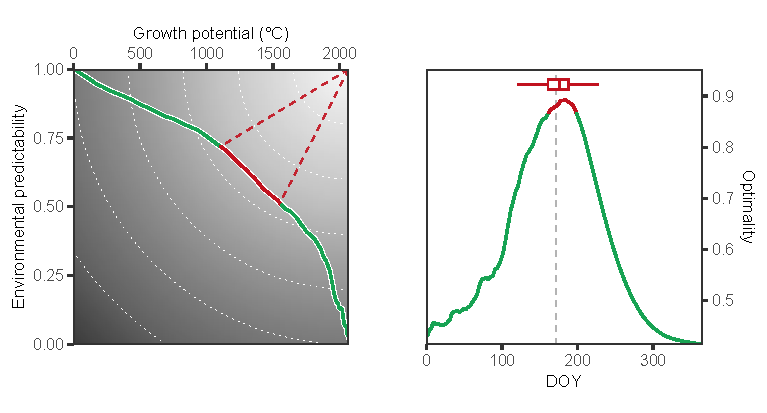
\includegraphics{global_optimality.pdf}
\vspace*{-0.5cm}
\caption{\textbf{Solstice marks the average optimal trade-off between environmental predictability and growth potential across Europe (1951-2020).} In the left panel, environmental predictability measures how well GDD by a given day predicts total yearly GDD ($R^2$ of a linear regression across years), while growth potential represents the remaining GDD from that day onward. In the right panel, optimality is based on the Euclidean distance from the (unattainable) perfect point where both predictability and growth potential are maximized (illustrated by the red dashed lines and the gray gradient in the left panel). The red sections of the green curves represent days where optimality falls within the 90th percentile (i.e. top 10\% most optimal days). GDD range was defined between 5\degree C and 35\degree C (see Figure S2 for 0-40\degree C).} 
\label{fig:globaloptimality}
\end{figure}

Using this trade-off framework, we found the optimal period to be near the summer solstice (\Cref{fig:globaloptimality}). Averaging across all of Europe, solstice appears as a critical juncture for the optimization of both environmental predictability and remaining growth potential.
% JDavies: "I think you need to explain this better, if plants want to optimise growth potential they should just keep on growing ..."
If this specific day indeed represents a broad-scale optimum across different climatic conditions, evolution towards a universal solstice trigger could make sense---especially since this optimum appears stable over the Holocene (Supplementary Figure S3). 

Our results suggest solstice could act as a reliable marker but also highlight the challenges in disentangling the influence of the solstice from that of a thermal optimum cue. %JDavies: Explain what s the support for this sentence.
% We show that solstice trades-off environmental predictability and growth potential, but 
Given our metrics are based only a thermal season---i.e. we do not explicitly incorporate a photoperiod driver---our results suggest the existence of an understudied thermal cue that could give the same outcome.
% DBuonaiuto: "Can you say this a bit more clearly? Walk us through what you mean here"
% does solstice coincide with the period of highest thermal energy in temperate regions? Peak of daily GDD is rather after solstice...
Plants could also rely on a combination of both solstice and thermal cues to optimize growth and reproductive timing---which would likely provide greater signal robustness to environmental change through partial redundancy between cues \citep{Bonamour2019}.
Alternatively, this overlap could simply represent an emergent property of the climate system that plants do not necessarily use as a cue, since it would be costly for plants to closely track two different signals---i.e. to encode and decode both thermal and photoperiod information within their cells. In this case, solstice may merely represent a climatic reality that summer temperatures are relatively stable year-to-year over July and August, and thus average GDD predictability peaks in late June. %emw19Jan -- I don't use contractions (do not instead of 'don't) or 'on one hand... on the other hand' in scientific writing

% \item Supporting this we found important variation over space (and time?)
%emw11Dec: I don't think cautionary is what we want ... depends on what you mean above. (If we need to toss the coincidence point above then I think we need to set up more in the end of the previous paragraph how this evolution would happen -- and at what scales perhaps.)
Supporting the hypothesis that solstice may not be a reliable cue, our results reveal substantial variation in the optimal timing when examined across Europe (\Cref{fig:localoptimality}), as opposed to averaging over space (\Cref{fig:globaloptimality}). In warmer southern Europe, plants reach an optimum earlier in the season, whereas in northern regions, cooler temperatures delay this timing beyond the solstice. 
% JDavies: "is there some way you can show plants in these regions don't use solstice?  I think I mentioned this to Lizzie earlier, but it would be great if you could show whether plants that were poorly predicted by solstice (in Zhoner et al. 2023) fall in regions where solstice is a poor predictor!"
This regional variability suggests that plants should likely 
%be partially adapted to their local climates---and especially to how GDD accumulate in their specific environment 
rely on cues that allow for a more plastic response in their specific environment than solstice would yield. 
From a parsimonious perspective, tracking primarily GDD-related cue might be more straightforward and aligned with the actual energy a plant needs to grow and reproduce---i.e. the cue would be sampled from a variable directly used by the plant.
 % (= directly linked to metabolic processes) i.e. the cue is sampled from a variable directly use by the plant
%emw11Dec: Recommend with stick with photoperiod or daylength across whole paper unless we're making an important distinction. 
Whereas tracking the solstice is likely more complex. Indeed, plants would need to sense not just the photoperiod but also the variation in the rate of change of photoperiod over time---essentially, the second derivative.
% more directly beneficial for the plant?
% What would be the benefit to have a separate mechanism, with the risk of a potential redundancy of tracking both the solstice and thermal cues? (but which thermal cue to track the optimal period?) => increase robustness of the signal with  partial redundancy bewteen cues


% Maybe we need to talk more about photoperiod cue sensing? What is known ("not a new result" Isabelle...) => make a paragraph?
% second derivative sensing seems unlikely, but we know photoperiod can be important?
% what could be the benefit of tracking photoperiod => synchronize populations broadly?
% if plants don't use solstice or if they don't use photoperiod, which cue(s) they need to track to understand that it is the optimal period, ? Temperature (and daily GDD accumulation) peaks after the optimum, so it should be something else?
% Does using solstice will prevent adaptative plasticity in future climate, ie plants could be "locked in a solstice response" (and mention supp figure with CMIP6 projections?)
% + "photosynthetic capacity peaks just after summer solstice and declines with decreasing photoperiod, before air temperatures peak" https://www.pnas.org/doi/10.1073/pnas.1119131109#fig02
% "In the most extreme cases, a new environment is generating a signal similar to a previously known cue, but completely uncorrelated with both the original cue and the environment of selection."


% \begin{enumerate}
%     \item critical need for experiments to disentangle daylength vs temp.
%     \item researchers need to more clearly test for (i) trends estimated at local scale across gradient and (ii) how they scale up to (sub)continental/global scales
% \end{enumerate}

%emw19Jan -- This last paragraph has gotten less strong over time, it feels less directly related to our results and more like stuff we could write at the end of lots of papers so I tried to pull it back to our results and make it shorter, see what you think. Also, if you keep this, fix how I just wrote in citations ... 
% vvdm19Jan: oow this feels so much nicer!
Taken together, our results suggest solstice could be an optimal signal for plants to transition key physiological processes when averaged across space, and appears remarkably stable over past and potential future climates  (Supplementary Figures S3 and S4), but is unstable at the local site-level (\Cref{fig:localoptimality}, Supplementary Figure S5). Because selection operates on individuals, this disconnect between the local and continental scales makes it difficult to understand how solstice would evolve as a trigger, and suggests its importance in correlative analyses (such as ours, \citet{Zohner2023} and \citet{Journe2024}) may appear due to natural correlations in environmental data that do not shape plant responses \citep[e.g.][]{Gao2024}. Alternatively, our results could suggest an understudied role of solstice in how plants sense photoperiod with potentially deep evolutionary origins \citep{morales2024phylogenetic}. Disentangling these two hypotheses will require new experiments that decouple natural covariation between temperature and photoperiod \citep{Buonaiuto2023, Elmendorf2020} to identify the cues plants use and more efforts to understand the fitness landscape of the growing season across space and time. %emw19Jan -- could probably cite something by Eric Post and/or John Park here OR check out Chevin and Lande 2015 perhaps? Or, you could cut this ending, which is a bit over the top perhaps. 

%emw19Jan -- leaving old text here ... 
\iffalse
Disentangling the role of the solstice as a cue for major growth and reproductive transitions is challenging, as plants have already started accumulating GDD several months before the solstice.
Complex natural correlations in environmental data may generate spurious results \citep[e.g.][]{Gao2024}, challenging us to test predictions from multiple avenues. % "inherent correlations in climate in regions that the field does not fully understand/incorporate"
Future research should explore which thermal cues might allow plants to track the optimal period, how these compare to a solstice-based cue, and whether they remain reliable in future climates (Supplementary Figures S4 and S5). %emw19Jan -- FYI, you can cross-reference you supp figures if you want with latex. You likely already know this, but if not, check out the labgit wiki on latex. 
% as daily GDD accumulation peak after solstice suggests the need for an alternative cue...?
To address this requires carefully designed experiments that decouple natural covariation between temperature and photoperiod \citep{Buonaiuto2023, Elmendorf2020} and integrate new understanding of the multiple ways plants sense photoperiod \citep{wang2024plants}.  
%emw11Dec: Hmm, I suspect there is a Korner or Basler paper we could cite instead of Dan's paper? 
%vvdm17Dec: do you have a specific paper in mind? this one: https://doi.org/10.1093/treephys/tpu021 ? (even though the focus is not on the covariation of temperature and photoperiod?)
Beyond small-scale experiments, understanding local-scale trends and how they scale up to subcontinental scales could help inform what trends plants may leverage to predict their environments over time. 
Ultimately, a better understanding of how plant responses to photoperiod and temperature vary regionally will help clarify broader biological patterns.
% =>  and finally: inform phenological models, allowing researchers to build more accurate predictions by incorporating the specific cues plants use to trigger growth
% JDavies: "reference to 'synchrony' comes out of nowhere ..."
\fi 

\begin{figure}[h]
% \centering
\hspace*{-1.2cm}
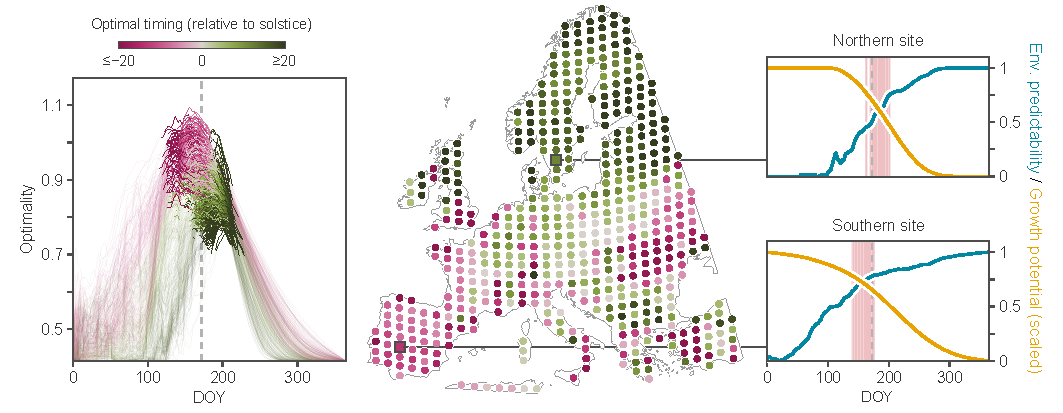
\includegraphics{local_optimality_alt.pdf}
\vspace*{-0.9cm} %emw19Jan -- I tried to spell out a little more this difference in optimal for the average versus for each site.
\caption{\textbf{Average optimal timing (\Cref{fig:globaloptimality}) hides variation in optimal timing across the different climatic conditions of Europe (1951-2020).} On the left panel, each curve shows the optimality for a given site. Sites are sampled on a regular grid across Europe, as shown on the central map. Colors indicate the timing---relative to the solstice---of the median optimal day. The two panels on the right show the trade-off between environmental predictability and growth potential (scaled to $[0,1]$) for two different sites. Days considered as optimal are highlighted in red.}
\label{fig:localoptimality}
\end{figure}

%\end{enumerate}
\clearpage

\bibliography{synchrony}

\end{document}
